\section{机制验证：受控消融如何支撑机制命题}
\label{sec:mechanism-tests}

本节把已有表格和图表组织成机制命题的检验。核心问题是：CLIP 局部响应如何通过图像条件化参照成为可靠异常证据？围绕这一问题，受控实验分别检验四个环节：直接局部线索是否足以成图，语义响应能否单独完成校准，局部可靠性如何改变 evidence selection，以及保守 calibration 是否维持正常图稳定。

\subsection{命题一：直接局部线索构成负控}

直接把局部可靠性图与初始语义响应融合，可以检验局部线索直接成图的机制假设。表~\ref{tab:controlled-core-ablation} 中 direct wavelet fusion 的像素级结果低于 baseline、semantic prototype adaptation 和最终方法：在 MVTec 上为 $88.7/80.4$，在 VisA 上为 $94.6/85.1$。这一负控说明，局部高频或结构变化本身提供候选区域；在本文机制中，它们进入 evidence selection，作为 prototype calibration 前的可靠性约束。图~\ref{fig:controlled-core-progression-cn} 给出从 baseline 到最终方法的顺序关系。

\begin{table*}[t]
\centering
\caption{Controlled core ablation on MVTec and VisA. All metrics are reported in percent; the best result within each dataset and metric is marked in bold.}
\label{tab:controlled-core-ablation}
\resizebox{\textwidth}{!}{%
\begin{tabular}{llcccc}
\toprule
Dataset & Variant & Pixel AUROC & Pixel AUPRO & Image AUROC & Image AP \\
\midrule
MVTec & Baseline & 91.2 & 83.2 & 91.6 & 96.4 \\
MVTec & Direct wavelet fusion / no adaptation & 88.7 & 80.4 & 92.9 & 96.9 \\
MVTec & GlobalRef & 91.2 & 84.3 & 93.1 & 96.9 \\
MVTec & Semantic prototype adaptation & 91.6 & 85.2 & 93.7 & 97.1 \\
MVTec & Ours w/o conservative update & 91.7 & 85.8 & 93.9 & 97.2 \\
MVTec & Ours (unnamed) & \textbf{91.8} & \textbf{86.2} & \textbf{94.1} & \textbf{97.4} \\
\midrule
VisA & Baseline & 95.5 & 86.7 & 82.0 & 85.3 \\
VisA & Direct wavelet fusion / no adaptation & 94.6 & 85.1 & 81.6 & 84.8 \\
VisA & GlobalRef & 95.8 & 89.2 & 83.2 & 86.4 \\
VisA & Semantic prototype adaptation & 96.0 & 90.4 & 83.7 & 86.9 \\
VisA & Ours w/o conservative update & 96.1 & 91.3 & 84.1 & 87.0 \\
VisA & Ours (unnamed) & \textbf{96.2} & \textbf{91.7} & \textbf{84.3} & \textbf{87.3} \\
\bottomrule
\end{tabular}%
}
\end{table*}


表中的行对应不同的可证伪预期。Baseline 检验固定 prototypes 下的初始语义响应；Direct wavelet fusion / no adaptation 检验局部可靠性图直接成图的效果；Semantic prototype adaptation 检验语义响应驱动的图像条件化校准，它是强对照；Ours w/o conservative update 检验可靠证据选择在缺少保守门控时的稳定性；最终 \method{} 同时使用语义先验、边界感知可靠性和保守校准。这个顺序使表~\ref{tab:controlled-core-ablation} 成为机制路径检验：分数随证据选择和校准机制逐步变好，而直接局部融合构成反向证据。

\begin{figure}[t]
  \centering
  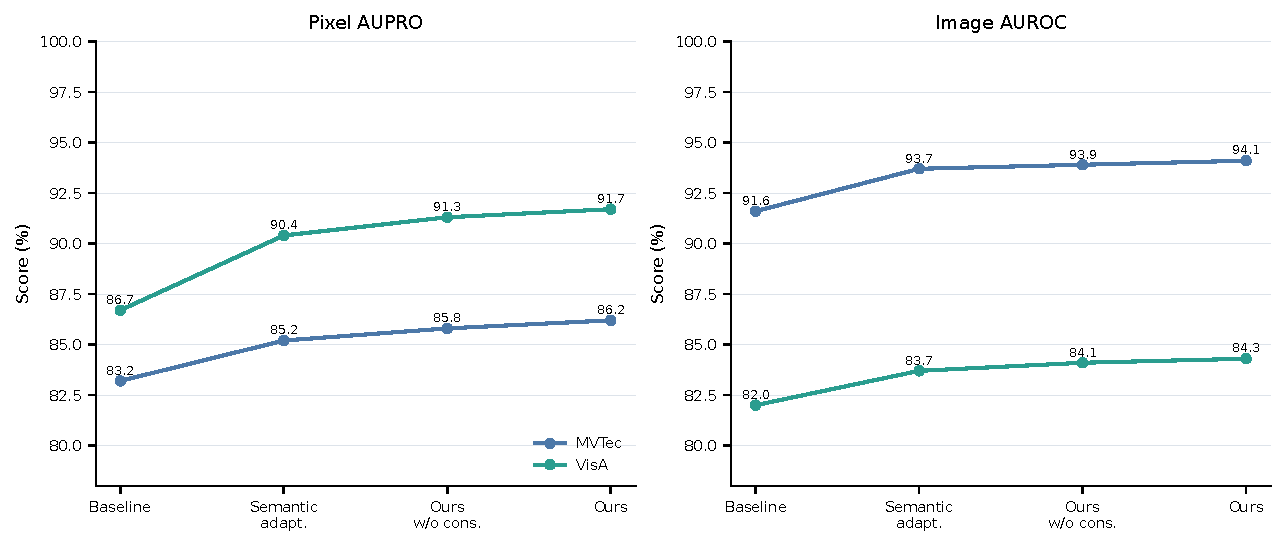
\includegraphics[width=\linewidth]{../paper/figures_ablation/figures/controlled_core_ablation_progression_lines.pdf}
  \caption{受控核心消融的顺序关系。该图验证机制路径：直接局部线索为负控，语义 prototype adaptation 是强对照，加入可靠局部证据和保守校准后形成最终方法。}
  \label{fig:controlled-core-progression-cn}
\end{figure}

\subsection{命题二：证据选择需要语义之外的局部可靠性}

以 $s_i^0$ 选择 normal/abnormal evidence 会继承 CLIP 初始语义响应的偏差。表~\ref{tab:wavelet-design-ablation} 将 semantic-only prototype adaptation、HF-only reliability、boundary-aware reliability 和最终保守校准放在同一受控路径中。该表支持两个判断：第一，局部可靠性进入 evidence selection 后，结果相对于 semantic-only 继续提升；第二，boundary-aware reliability 在像素级 AUPRO 上相对于 HF-only 更稳定，符合“高频线索需要排除结构边界解释”的机制假设。

\begin{table*}[t]
\centering
\caption{Wavelet reliability design ablation on MVTec and VisA. All metrics are reported in percent; the best result within each dataset and metric is marked in bold.}
\label{tab:wavelet-design-ablation}
\resizebox{\textwidth}{!}{%
\begin{tabular}{llcccc}
\toprule
Dataset & Variant & Pixel AUROC & Pixel AUPRO & Image AUROC & Image AP \\
\midrule
MVTec & Direct wavelet fusion & 88.7 & 80.4 & 92.9 & 96.9 \\
MVTec & Semantic-only prototype adaptation & 91.6 & 85.2 & 93.7 & 97.1 \\
MVTec & HF-only reliability + prototype adaptation & 91.6 & 85.3 & 94.0 & 97.2 \\
MVTec & Boundary-aware reliability + prototype adaptation & 91.7 & 85.7 & 93.8 & 97.3 \\
MVTec & Ours (unnamed) & \textbf{91.8} & \textbf{86.2} & \textbf{94.1} & \textbf{97.4} \\
\midrule
VisA & Direct wavelet fusion & 94.6 & 85.1 & 81.6 & 84.8 \\
VisA & Semantic-only prototype adaptation & 96.0 & 90.4 & 83.7 & 86.9 \\
VisA & HF-only reliability + prototype adaptation & 96.0 & 90.8 & 84.0 & 86.9 \\
VisA & Boundary-aware reliability + prototype adaptation & 96.1 & 91.2 & 83.9 & 87.1 \\
VisA & Ours (unnamed) & \textbf{96.2} & \textbf{91.7} & \textbf{84.3} & \textbf{87.3} \\
\bottomrule
\end{tabular}%
}
\end{table*}


更具体地，高频可靠性行检验“原始高频是否足够作为证据选择信号”；边界感知可靠性行检验“抑制低频结构边界后，证据选择是否更符合参照估计假设”；最终 \method{} 进一步检验“可靠证据选择与保守 prototype calibration 配套后是否形成稳定参照”。因此，表~\ref{tab:wavelet-design-ablation} 的作用是区分三种机制解释：直接局部变化、语义自校准、以及语义先验约束下的边界感知证据选择。

\begin{figure}[t]
  \centering
  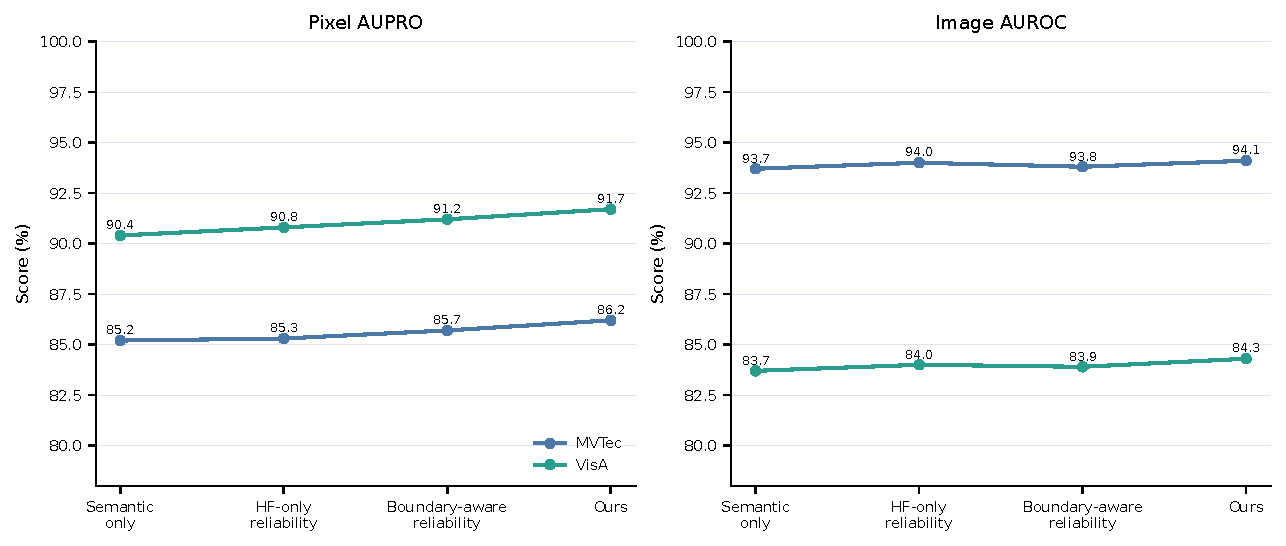
\includegraphics[width=\linewidth]{../paper/figures_ablation/figures/wavelet_design_ablation_progression_lines.pdf}
  \caption{局部可靠性设计消融。该图检验证据选择机制：semantic-only 使用初始语义响应，HF-only 引入原始局部变化，boundary-aware 进一步抑制结构边界混淆，最终方法加入保守 prototype 校准。}
  \label{fig:wavelet-design-progression-cn}
\end{figure}

\subsection{命题三：参照校准必须保守}

图像条件化参照需要控制错误证据写入。当前稳定设置令异常侧保持原 prototype，并采用受置信度缩放和门控约束的小步正常侧校准。正常图稳定性验证支持这一选择：相对于 baseline，最终方法的正常图误报面积更低。表~\ref{tab:normal-stability-cn} 汇总了已记录的正常图统计，MVTec 的 p95/p99 FP area 从 $5.002/1.001$ 降至 $4.895/0.960$，VisA 从 $4.996/1.001$ 降至 $4.718/0.937$。

\begin{table}[t]
  \centering
  \caption{正常图稳定性。FP area 表示在正常图上超过对应阈值的面积比例，越低越好。该表检验保守校准对正常图误报面积的影响。}
  \label{tab:normal-stability-cn}
  \resizebox{\linewidth}{!}{%
  \begin{tabular}{llccc}
    \toprule
    Dataset & Method & Normal images & FP area @ p95 & FP area @ p99 \\
    \midrule
    MVTec & Baseline & 467 & 5.002\% & 1.001\% \\
    MVTec & \method{} & 467 & 4.895\% & 0.960\% \\
    VisA & Baseline & 962 & 4.996\% & 1.001\% \\
    VisA & \method{} & 962 & 4.718\% & 0.937\% \\
    \bottomrule
  \end{tabular}%
  }
\end{table}

\subsection{命题四：系统级结果与机制结论分层对应}

已有五数据集结果和 ICONIP-style baseline 表格展示系统级表现；上述受控机制验证支撑本文的机制命题。对于 MVTec/VisA，受控表检验的是 \method{} 相对于 semantic-only / direct fusion 的机制路径；对于 MPDD、BTAD 和 DTD-Synthetic，当前结果包含 system-level 设置，并区分 global setting 与 dataset-tuned upper bound。五数据集表适合回答完整系统在不同数据集上的表现，本节的受控表负责回答机制来源。

这一分层对应两类证据功能：包含 multi-crop 或 pixel-to-image calibration 的系统级行展示完整系统表现；受控消融解释 prototype-reference 机制。本文的机制 claim 由受控消融支撑：direct local cue scoring 是负控，semantic-only calibration 是强对照，可靠局部证据与保守图像条件化参照共同构成最终方法。由此，表格和图形成一条连续证据链：候选局部线索先被证伪为直接异常图，再作为 evidence selection 约束进入参照估计，最后通过正常图稳定性验证其校准幅度。
